\documentclass[a4paper,fontsize=11pt, line_length=42zw,number_of_lines=35,gutter=15mm]{jlreq}
\renewcommand{\baselinestretch}{1.1}

\usepackage{graphicx}
\usepackage{xcolor}
\usepackage[cmex10]{amsmath}
\usepackage{booktabs}
\usepackage{ascmac}
\usepackage{amssymb}
\usepackage{caption}
\usepackage{colortbl}
\usepackage{float}
\usepackage{textcomp}
\usepackage[breaklinks=true, pdfborder={0 0 0}]{hyperref}
\usepackage{enumitem}
\usepackage[style=ieee,backend=biber]{biblatex}
\addbibresource{refs.bib}

\setcounter{tocdepth}{3}

\title{技術文書作成 期末試験レポート \\
  \large 非線型方程式の数値解法の収束速度比較}
\author{26G1012\quad 石井陽泰}
\date{\today}

\begin{document}
\maketitle

\section{はじめに}

\section{手法}

\subsection{方程式の説明}
本レポートで対象とする方程式は以下:
\begin{equation}
  f(x)=\cos(x)-x^2
  \label{eq:fn_f}
\end{equation}
方程式(\ref{eq:fn_f})の解を求めるにあたり, まず関数$f(x)$のグラフを描くことで, 解の存在範囲を確認する.

\begin{figure}[h]
  \centering
  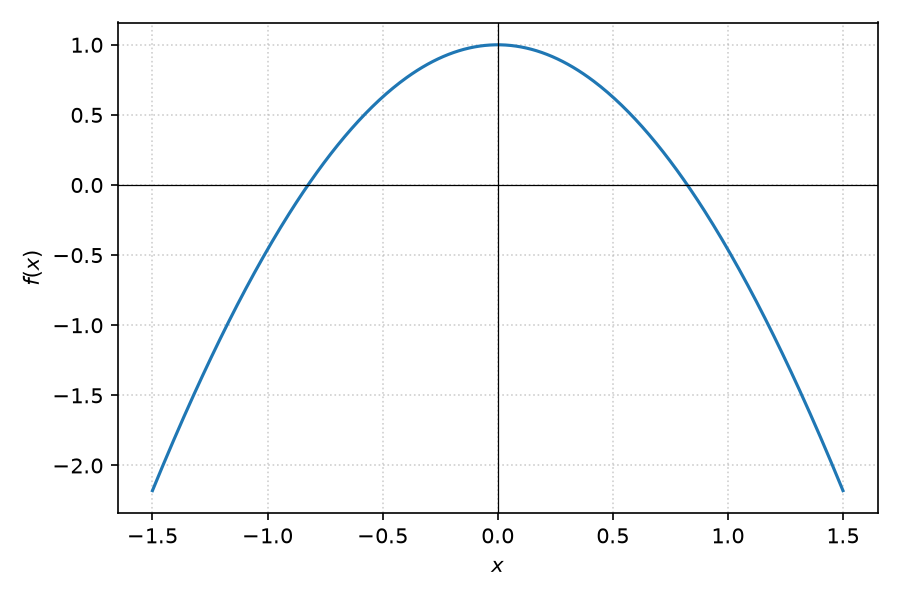
\includegraphics[width=12cm]{./data/fig_fx.png}
  \caption{関数$f(x)=\cos(x)-x^2$のグラフ}
  \label{fig:fn_f}
\end{figure}
図\ref{fig:fn_f}に$y=f(x)$の曲線を示す. 
図\ref{fig:fn_f}より, 方程式(\ref{eq:fn_f})の解は, 区間 $0.5<x<1$ および $-1<x<-0.5$ 内にそれぞれ 1 つずつ存在することがわかる.

さらに, 関数 $f(x)=\cos(x)-x^2$ は偶関数であり, 任意の $x$ に対して $f(-x)=f(x)$ が成り立つため, グラフは $y$ 軸に関して対称である. 
したがって, 正の側に零点 $x^*>0$ が存在すれば, 負の側にはその符号を反転させた点 $-x^*$ が自動的に零点として対応する. 
本レポートではこの対称性に着目し, 数値解法の適用対象を正の側の零点 $x^*\in(0.5,1)$ 一つに限定したうえで, その近似解を求めることにする.

\subsection{非線形方程式の求解の手法}
本節では, 対象方程式(\ref{eq:fn_f})のように解析的に解けない非線形方程式に対して, 数値的に近似解を求める手法を扱う. 
ここでは, 二分法\ref{sbsbsec:bisec}とニュートン法\ref{sbsbsec:newton}について, その原理を述べたうえで漸化式またはアルゴリズムを導出する. 

\subsubsection{二分法の原理・漸化式・アルゴリズム}
\label{sbsbsec:bisec}
本節では, 連続関数 $f(x)$ に対して方程式\ref{eq:fn_f}を解く二分法を, 平均値の定理に基づく原理から説明し, 
その漸化式およびアルゴリズムを導出する. 
まず, 連続関数 $f(x)$ について, $f(a)f(b)<0$ を満たす区間 $[a,b]$ が与えられていると仮定する. 
このとき, 連続性と中間値の性質より, 端点で符号が異なることから区間内に少なくとも1つの零点 $x^*$ が存在することが保証される. 
この零点の存在に関する結果は, 19 世紀初頭に Bolzano によって解析的に証明されたことでも知られている. \cite{bernardReinAnalytischerBeweis1817}
すなわち, $a<x^*<b$ を満たす点で $f(x^*)=0$ が成り立つ. 二分法はこの「区間両端で符号が異なればその内部に零点が存在する」という原理に基づいて, 
常に零点を含む側の半区間のみを残す操作を繰り返すことで, 解の存在区間を段階的に絞り込む手法である. 
具体的には, $n$ 回目の反復で零点を含む区間 $[a_n,b_n]$ が得られているとき, 
中点を $c_n=(a_n+b_n)/2$ と定義し, 関数値 $f(c_n)$ の符号を調べる. 
もし $f(a_n)f(c_n)<0$ であれば零点は $[a_n,c_n]$ 内に存在するので, 
次の区間を $[a_{n+1},b_{n+1}]=[a_n,c_n]$ に更新する. 
そうでなければ（$f(a_n)f(c_n)\ge 0$ であれば）零点は $[c_n,b_n]$ 内に存在するので, 
$[a_{n+1},b_{n+1}]=[c_n,b_n]$ と更新する. 
関数の連続性と中間値の性質により, 各反復後の区間 $[a_{n+1},b_{n+1}]$ もなお零点を含むため, 
この操作を区間幅や関数値が所定の収束条件を満たすまで反復することで近似解を得ることができる. 
二分法では, 各反復で区間を正確に半分に縮めるため, 区間幅 $L_n=|b_n-a_n|$ は漸化式 $L_{n+1}=\tfrac{1}{2}L_n$ を満たす. 
初期区間幅を $L_0=|b_0-a_0|$ とおくと, これを繰り返し適用することで $L_n=\dfrac{|b_0-a_0|}{2^n}$ と表される. 
したがって, $n$ 回目の反復後の区間幅は $|b_n-a_n|=\dfrac{|b_0-a_0|}{2^n}$ となり, 目標とする精度に必要な反復回数をこの式から見積もることができる. 

\subsubsection{ニュートン法の原理・漸化式・アルゴリズム}
\label{sbsbsec:newton}
本節では, 連続微分可能な関数 $f(x)$ に対して方程式~\eqref{eq:fn_f} を解くニュートン法を, 接線近似に基づく原理から説明し, 
その漸化式およびアルゴリズムを導出する. 
ニュートン法の起源は, Isaac Newton による未刊草稿\emph{De Analysi per Aequationes Numero Terminorum Infinitas}（1669）にさかのぼり, \cite{newtonAnalysiAequationesNumero1669}
その手法が初めて印刷物として広く公刊されたのはWallis の代数学書 \emph{A Treatise of Algebra, both Historical and Practical}（1685）とされる. \cite{wallisTreatiseAlgebra1685}
同書では方程式の近似解を求める反復的手続きが述べられており, 後に Newton--Raphson 法として確立された方法の原型が見られる. 

いま, 求めたい解 $x^*$ が $f(x^*)=0$ を満たすとする. ニュートン法は, 
現時点の近似解 $x_n$ の近傍で $f(x)$ を 1 次のテイラー展開によって線形近似し, 
この直線近似の零点を次の近似値として更新するという原理に基づく. 
すなわち, $x_n$ の近傍で
$$f(x) \approx f(x_n) + f'(x_n)(x-x_n)$$
と近似し, 右辺を 0 とおいて解くと, 
$$f(x_n) + f'(x_n)(x_{n+1}-x_n) = 0$$
より, 
$$x_{n+1} = x_n - \frac{f(x_n)}{f'(x_n)}$$
という漸化式が得られる. 
この更新式は「現在の点 $x_n$ におけるグラフの接線を $x$-軸と交わるまで延長し, 
その交点を次の近似解 $x_{n+1}$ とする」という幾何学的解釈を持ち, 
Wallis の著作でもこのような接線に基づく逐次近似の考え方が現れている.\cite{wallisTreatiseAlgebra1685}

一般に, 初期値 $x_0$ の選び方と関数 $f$ の性質に適切な条件（例えば, 
$x^*$ の近傍で $f$ が十分滑らかであり, $f'(x^*)\neq 0$ を満たすこと）を課すとき, 
ニュートン法の反復列 $\{x_n\}$ は真の解 $x^*$ に向かって収束し, 
さらに誤差はおおよそ 2 乗で減少する, すなわち 2 次収束することが知られている. 
具体的なアルゴリズムとしては, 初期値 $x_0$ を与えたのち, 
各反復 $n=0,1,2,\dots$ で
$$x_{n+1} = x_n - \frac{f(x_n)}{f'(x_n)}$$
を計算し, $|x_{n+1}-x_n|$ や $|f(x_{n+1})|$ が所定の収束判定条件を満たした時点で反復を終了し, $x_{n+1}$ を近似解とみなす. 
このようにニュートン法は, 接線近似という単純な幾何学的原理に基づきつつ, 
適切な条件のもとでは二分法よりもはるかに速い 2 次収束を達成する強力な反復解法である. 

\subsection{プログラムの仕様}
\subsubsection{環境}
\subsection{評価指標}
本報告書では, 非線形方程式の近似解を与える両手法の収束の速さを, 許容誤差を満たすまでに要した反復回数によって評価する. 
具体的には, 正の側の零点 $x^*$ に対する近似解が許容誤差 $\varepsilon = 10^{-8}$ を満たすまで反復を続けたときの反復回数 $n$ を収束の速さの評価指標として一意に定める.
二分法とニュートン法を同一条件下で比較するため, 両手法とも同じ方程式 $f(x)=\cos(x)-x^2$ を対象とし,
同じ零点 $x^*$ に収束するように初期区間および初期値を設定したうえで, この評価指標 $n$ を用いて結果を集計する.

\section{結果}
\section{おわりに}
% \section{はじめに}
% 近年, スーパーマーケット業界では, 人口減少や節約志向の強まりに加え, ドラッグストアやECとの競合激化により客数の伸びが鈍化し, 
% 既存店舗の売上が頭打ちとなっていることが指摘されている. 

% しかしながら, どのような店舗要因が売上に影響しているのかは十分に明らかになっていない. 

% 本レポートでは, 滋賀県で10店舗を展開するCITスーパーにおける売上高の減少要因を分析する.
% 本レポートの目的は, 各店舗のアンケート結果と売上高のデータから売上低下の主因を特定し, 最も効率的に売上を改善するための施策を提示することにある. 

% % ===========================================================
% \section{手法}
% \subsection{各店舗における売上高とスコア群}
% 本節では, 検討されるデータを示す.

% CITスーパーにおける, アンケート結果を\ref{tab:store_scores}に示す. 
% アンケートは各店舗の顧客から収集され, それぞれの項目（接客・品揃え・立地）に対して①から⑤のスコアを付与する.
% 満足度スコアは表\ref{tab:satisfaction}のように定義される:
% \begin{table}[htbp]
%   \centering
%   \caption{満足度スコアの定義}
%   \begin{tabular}{c|c}
%     スコア & 満足度 \
%     \hline
%     ① & 非常に不満 \
%     ② & 不満 \
%     ③ & 普通 \
%     ④ & 満足 \
%     ⑤ & 非常に満足 \
%   \end{tabular}

%   \label{tab:satisfaction}
% \end{table}

% \begin{table}[htbp]
%   \centering
%   \caption{店舗別スコアと売上高}
%   \label{tab:store_scores}
%   \begin{tabular}{ccccc}
%     \hline
%     店舗 & 接客スコア & 品揃えスコア & 立地スコア & 売上高（億円） \
%     \hline
%     A & 3.42 & 4.03 & 2.22 & 305.29 \
%     B & 4.49 & 4.07 & 1.84 & 281.99 \
%     C & 4.71 & 2.54 & 4.76 & 382.03 \
%     D & 0.39 & 3.11 & 3.62 & 346.11 \
%     E & 2.14 & 1.59 & 2.81 & 322.68 \
%     F & 4.67 & 4.63 & 1.63 & 277.73 \
%     G & 4.92 & 2.90 & 4.68 & 372.33 \
%     H & 4.13 & 2.85 & 2.69 & 314.68 \
%     I & 0.61 & 4.61 & 4.38 & 365.65 \
%     J & 3.78 & 3.10 & 4.28 & 357.50 \
%     \hline
%   \end{tabular}
% \end{table}

% \subsection{評価指標}
% 本節では, アンケート結果（接客・品揃え・立地）と各店舗の売上高との線形関係を明らかにするため評価指標を定義する.

% \ref{tab:store_scores}に対する評価指標として, 
% \begin{enumerate}[align=left, itemindent=2em, listparindent=\parindent, topsep=0.15em]
%   \item 回帰係数, 回帰残差
%   \item ピアソンの相関係数
% \end{enumerate}
% を用いる. 回帰係数$\hat{a}$, 回帰直線, 回帰残差$e_i$はそれぞれ以下のように定義される:
% \begin{equation}
%   (\hat{a}, \hat{b})
%   = \arg\min_{a,b} \sum_{i=1}^{n} \left( y_i - (a x_i + b) \right)^2
% \end{equation}

% \begin{equation}
%   \hat{y}_i = \hat{a} x_i + \hat{b}
% \end{equation}

% \begin{equation}
%   e_i = y_i - \hat{y}_i = y_i - (\hat{a} x_i + \hat{b})
% \end{equation}

% ピアソンの相関係数は以下:
% \begin{equation}
%   r
%   = \frac{
%       \displaystyle \sum_{i=1}^{n}
%       (x_i - \bar{x})(y_i - \bar{y})
%     }{
%       \displaystyle
%       \sqrt{
%         \sum_{i=1}^{n} (x_i - \bar{x})^2
%       }
%       \sqrt{
%         \sum_{i=1}^{n} (y_i - \bar{y})^2
%       }
%     }
% \end{equation}
% ここで$y$系列は\ref{tab:store_scores}における"売上高（億円）"列であり, $x$系列は"接客スコア", "品揃えスコア", "立地スコア"それぞれから選ぶ.

% \subsection{環境}
% 本説では散布図, 回帰, 相関の計算および表示に使用したソフトウェアとそのバージョンを示す.
% \begin{itemize}
%   \item Google Colaboratory
%   \item Python 3.12.13
%   \item pandas 2.2.2
%   \item matplotlib 3.10.0
% \end{itemize}

% % ===========================================================
% \section{結果}
% \label{sec:results}
%   % 作成した散布図を貼り付け, 読み取れることを説明する. 
%   % 下の figure 環境のコメントを外し, 自分で保存した図に差し替えること. 
% 図\ref{fig:scatter}に各種スコアと売上高の散布図を示す. 

% \begin{figure}[htbp]
%     \centering
%     \includegraphics[width=12cm]{./data/scatter.png}
%     \caption{各種スコアと売上高の散布図. }
%     \label{fig:scatter}
%   \end{figure}

% 図\ref{fig:scatter}から, 特に「立地」のスコアと売上高の間に強い正の相関が見られる一方で,
% 「接客」や「品揃え」のスコアは売上高との相関が相対的に低い,
% あるいは特定の範囲で頭打ちになる傾向があることが読み取れる.

% \section{おわりに}
% 本報告書では, 売上高を効率よく上昇させる要因を特定し施作に活かすため, 
% CITスーパー各店舗における, 接客・品揃え・立地をスコアリングするアンケートの結果と, 売上高の関係について, 散布図を用いた相関回帰分析を行なった.
% その結果, 接客スコア・品揃えスコア・立地スコアの中で, 立地スコアで最も強い売上高との相関関係, 最も大きな回帰係数, 最も少ない残差が観察された. 

% したがって, 売上高の改善に最も効果的な施策は「立地」の改善であると考えられる.
% 擬似相関の可能性を考慮しても, 立地のスコアが高い店舗は売上高も高い傾向が,
% 企業の出店戦略や地域の発展に沿った営業経緯など再現されない交絡因子を考えても
% 極めて顕著であるため, 新規店舗の出店や既存店舗の移転を検討することが有効である.
% 一方で, 「接客」や「品揃え」の改善も重要であるが,
% これらは売上高に対する影響が限定的である可能性がある.
% ただし立地の改善に比してコストがかかりづらいため, 優先順位を考慮する必要がある.

% 交絡分析や顧客セグメントごとの傾向を調査することで,
% 施策のコストパフォーマンスを検討することが課題として残るものの, 
% アンケート結果と売上高の関係の相関回帰分析から, 立地スコアを改善させる取り組みにより, 
% 売上高を効率よく上昇させられると考えられる.

\printbibliography[title=参考文献]
\end{document}